\documentclass[xetex,mathserif,serif]{beamer}
\usepackage{polyglossia}
\setdefaultlanguage[babelshorthands=true]{russian}
\usepackage{minted}
\usepackage{tabu}
\usepackage{moresize}

\useoutertheme{infolines}

\usepackage{fontspec}
\setmainfont{FreeSans}
\newfontfamily{\russianfonttt}{FreeSans}

\definecolor{links}{HTML}{2A1B81}
\hypersetup{colorlinks,linkcolor=,urlcolor=links}

\setbeamertemplate{blocks}[rounded][shadow=false]

\setbeamercolor*{block title alerted}{fg=red!50!black,bg=red!20}
\setbeamercolor*{block body alerted}{fg=black,bg=red!10}

\tabulinesep=1.2mm

\title{Базы данных}
\author[Юрий Литвинов]{Юрий Литвинов\\\small{\textcolor{gray}{yurii.litvinov@gmail.com}}}
\date{08.11.2019г}

\newcommand{\attribution}[1] {
\vspace{-5mm}\begin{flushright}\begin{scriptsize}\textcolor{gray}{\textcopyright\, #1}\end{scriptsize}\end{flushright}
}

\begin{document}

	\frame{\titlepage}

	\section{Введение}

	\begin{frame}
		\frametitle{СУБД}
		\begin{itemize}
			\item Реляционные
			\begin{itemize}
				\item Отношения
				\item Операции
			\end{itemize}
			\item Объектно-ориентированные
			\begin{itemize}
				\item Сериализованные объекты
			\end{itemize}
			\item Иерархические
			\item ...
		\end{itemize}
	\end{frame}

	\begin{frame}
		\frametitle{Реляционные vs ОО-СУБД}
		\begin{itemize}
			\item Реляционные
			\begin{itemize}
				\item Сложность интеграции с ОО-кодом
				\begin{itemize}
					\item ORM (Microsoft Entity Framework, Hibernate, MyBatis, ...)
				\end{itemize}
				\item Эффективные и выразительные запросы
			\end{itemize}
			\item Объектно-ориентированные
			\begin{itemize}
				\item Проще, легковеснее, не требуют ORM
				\item ``Бедный'' язык запросов
				\item Часто не умеют того, что для реляционных СУБД естественно (например, транзакций)
			\end{itemize}
		\end{itemize}
	\end{frame}

	\section{Реляционная модель данных}

	\begin{frame}
		\frametitle{Реляционная модель данных}
		\begin{center}
			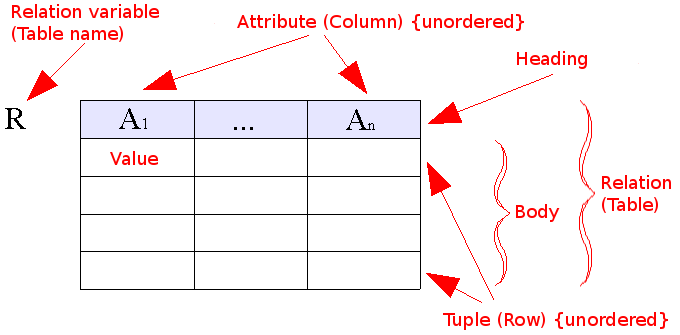
\includegraphics[width=0.9\textwidth]{relationalModel.png}
			\attribution{Wikipedia}
		\end{center}
	\end{frame}

	\begin{frame}
		\frametitle{Пример таблицы}
		\begin{center}
			\begin{tabu} {| X[0.9 l p] | X[1 l p] | X[1 l p] | X[1 l p] |}
				\tabucline-
				CustomerID       & TaxID        & Name       & Address           \\
				\tabucline-
				\everyrow{\tabucline-}
				1234567890       & 555-5512222  & Munmun     & 323 Broadway      \\
				2223344556       & 555-5523232  & Wile E.    & 1200 Main Street  \\
				3334445563       & 555-5533323  & Ekta       & 871 1st Street    \\
				423242432        & 555-5325523  & E.F. Codd  & 123 It Way        \\
			\end{tabu}
		\end{center}
	\end{frame}

	\begin{frame}
		\frametitle{Ключи}
		\begin{columns}
			\begin{column}{0.5\textwidth}
			\begin{itemize}
				\item Первичные (primary)
				\begin{itemize}
					\item Естественные
					\begin{itemize}
						\item Составные
					\end{itemize}
					\item Суррогатные
				\end{itemize}
				\item Внешние (foreign)
			\end{itemize}
			\end{column}
			\begin{column}{0.5\textwidth}
				\begin{scriptsize}
					CITY
					\begin{tabu} {| X[0.2 l p] | X[1 l p] |}
						\tabucline-
						ID      & Name \\
						\tabucline-
						\everyrow{\tabucline-}
						1       & Москва \\
						2       & Санкт-Петербург \\
						3       & Владивосток \\
					\end{tabu}
					\vspace{3mm}
					STREET
					\begin{tabu} {| X[0.2 l p] | X[1 l p] | X[0.7 l p] |}
						\tabucline-
						ID       & Name             & ID\_CITY \\
						\tabucline-
						\everyrow{\tabucline-}
						181      & Малая Бронная    & 1 \\
						182      & Тверской Бульвар & 1 \\
						183      & Невский проспект & 2 \\
						184      & Пушкинская       & 2 \\
						185      & Светланская      & 3 \\
						186      & Пушкинская       & 3 \\
					\end{tabu}
				\end{scriptsize}
			\end{column}
		\end{columns}
	\end{frame}

	\begin{frame}
		\frametitle{Ограничения}
		\begin{itemize}
			\item PRIMARY KEY
			\item FOREIGN KEY
			\item NOT NULL
			\item UNIQUE
			\item ...
		\end{itemize}
	\end{frame}

	\begin{frame}
		\frametitle{SQL SELECT}
		\begin{center}
			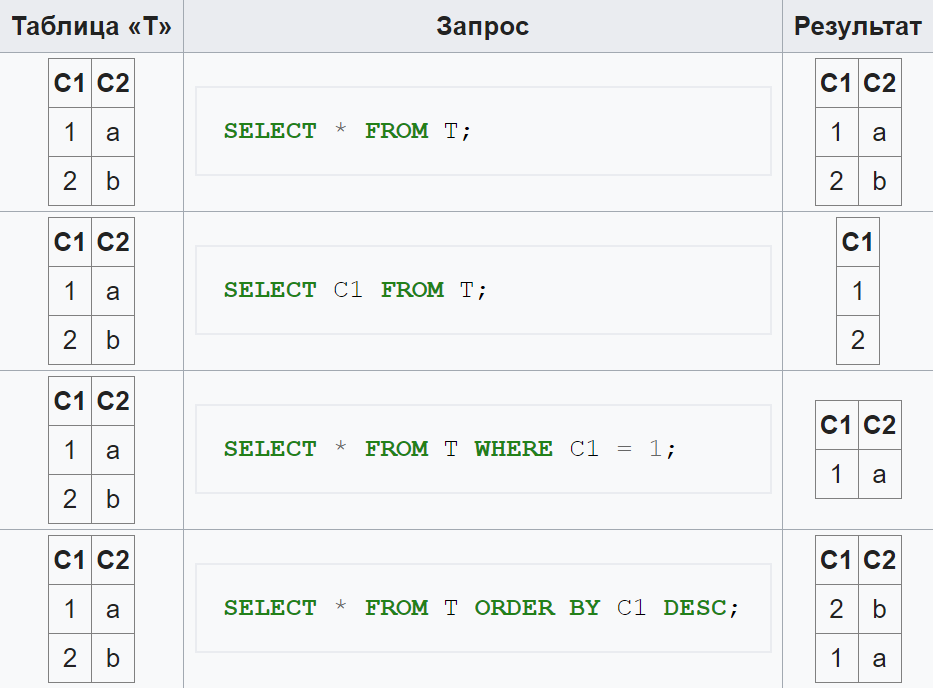
\includegraphics[width=0.7\textwidth]{select.png}
			\attribution{Wikipedia}
		\end{center}
	\end{frame}

	\begin{frame}[fragile]
		\frametitle{SELECT, вложенные запросы}
		\begin{minted}{sql}
SELECT isbn,
       title,
       price
FROM Book
WHERE price < (SELECT AVG(price) FROM Book)
ORDER BY title;
		\end{minted}
	\end{frame}

	\begin{frame}
		\frametitle{INNER JOIN}
		\begin{center}
			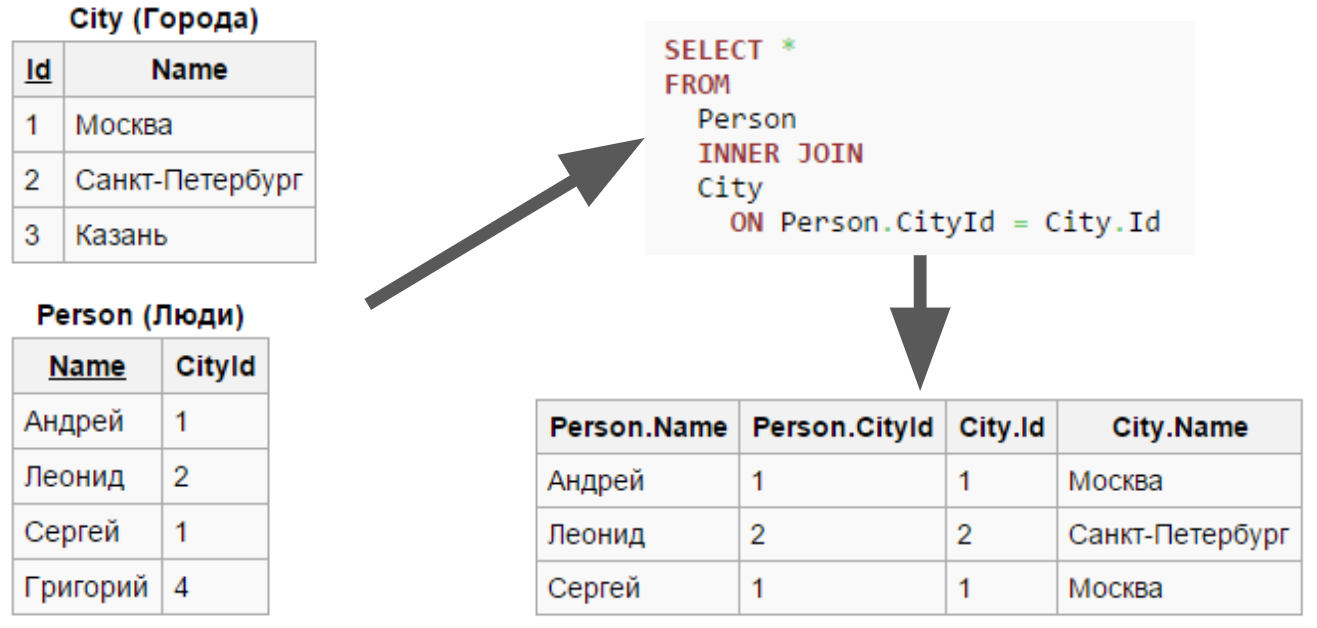
\includegraphics[width=0.9\textwidth]{innerJoin.png}
			\attribution{Wikipedia}
		\end{center}
	\end{frame}

	\begin{frame}
		\frametitle{OUTER JOIN}
		\begin{center}
			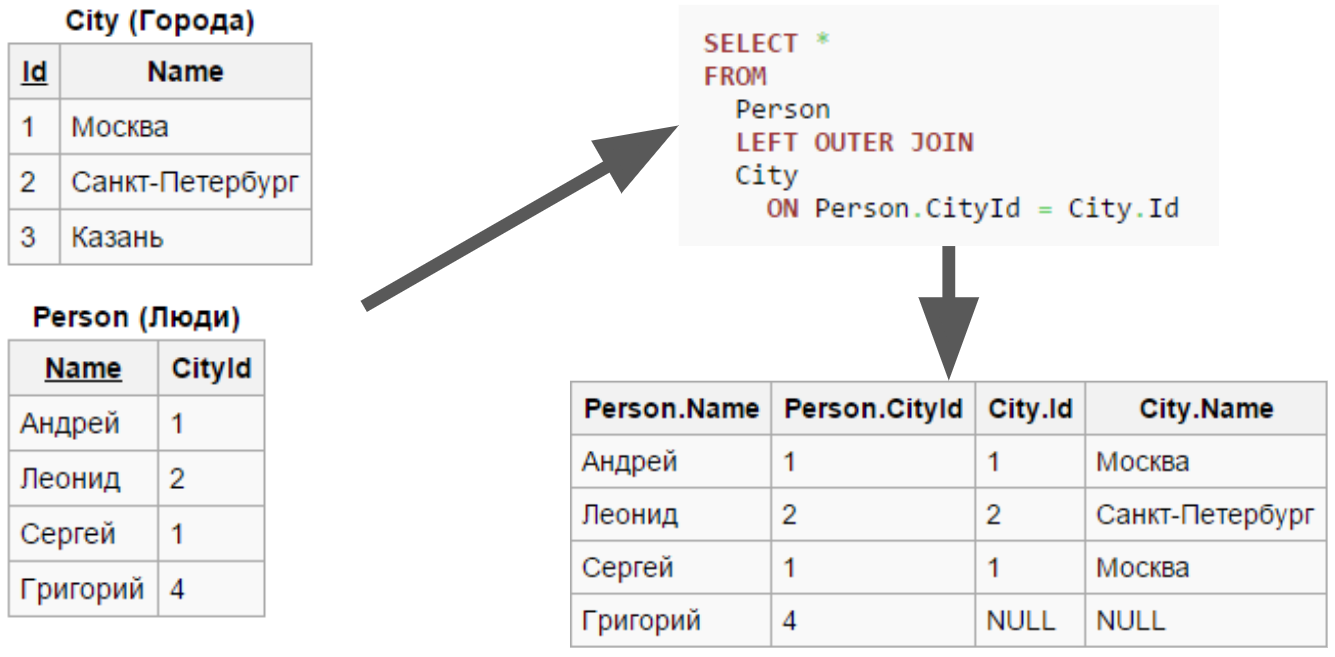
\includegraphics[width=0.9\textwidth]{outerJoin.png}
			\attribution{Wikipedia}
		\end{center}
	\end{frame}

	\begin{frame}
		\frametitle{CROSS JOIN}
		\begin{center}
			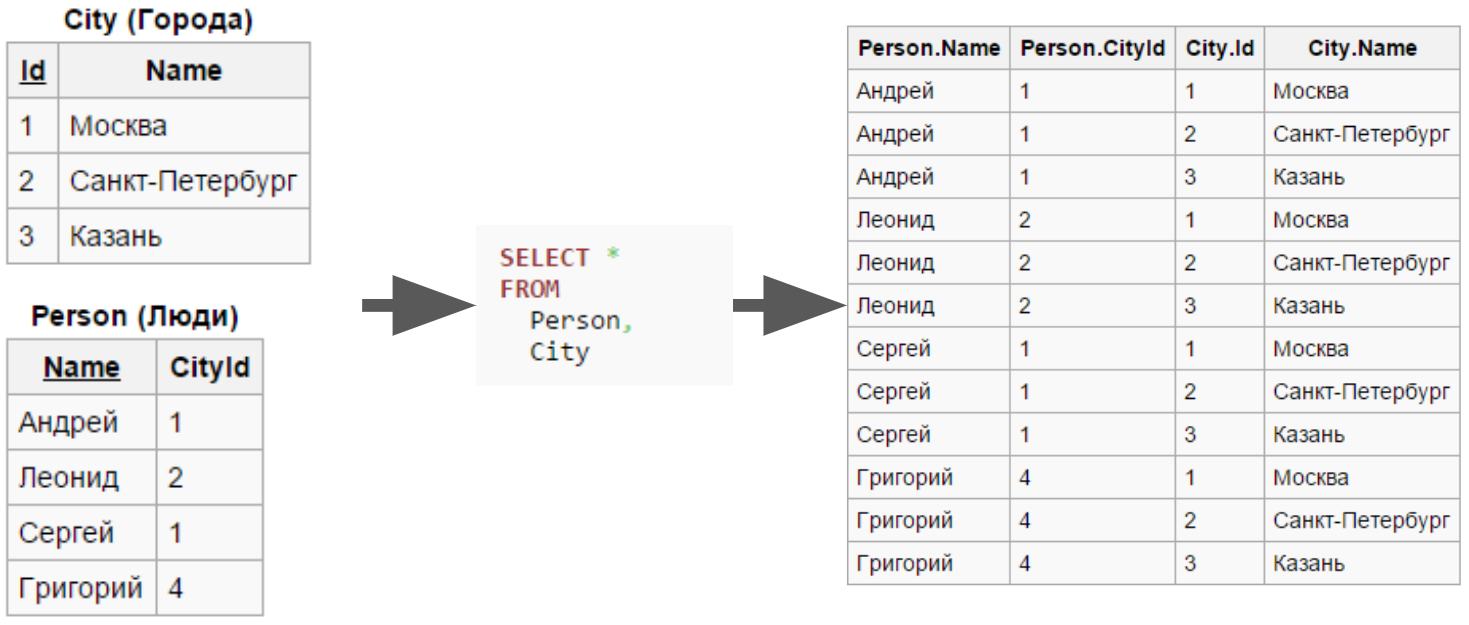
\includegraphics[width=0.9\textwidth]{crossJoin.png}
			\attribution{Wikipedia}
		\end{center}
	\end{frame}

	\begin{frame}[fragile]
		\frametitle{INSERT, UPDATE, DELETE}
		\begin{small}
			INSERT:
			\begin{minted}{sql}
INSERT INTO phone_books VALUES ('Peter Doe', '555-2323');
			\end{minted}

			\vspace{3mm}
			UPDATE:
			\begin{minted}{sql}
UPDATE persons SET
        street = 'Nissestien 67',
        city = 'Sandnes',
    WHERE lastname = 'Tjessem' AND firstname = 'Jakob';
			\end{minted}

			\vspace{3mm}
			DELETE:
			\begin{minted}{sql}
DELETE ab, b
    FROM Authors AS a, AuthorArticle AS ab, Articles AS b
    WHERE a.AuthID = ab.AuthID AND ab.ArticleID = b.ArticleID
        AND AuthorLastName = 'Henry';
			\end{minted}
		\end{small}
	\end{frame}

	\begin{frame}[fragile]
		\frametitle{Работа с метаинформацией}
		\begin{small}
			CREATE TABLE:
			\begin{minted}{sql}
CREATE TABLE Students (
    Code INTEGER NOT NULL,
    Name NCHAR(30) NOT NULL,
    Address NVARCHAR(50),
    Mark DECIMAL);
			\end{minted}

			\vspace{3mm}
			DROP TABLE:
			\begin{minted}{sql}
DROP TABLE Students;
			\end{minted}
		\end{small}

		\begin{center}
			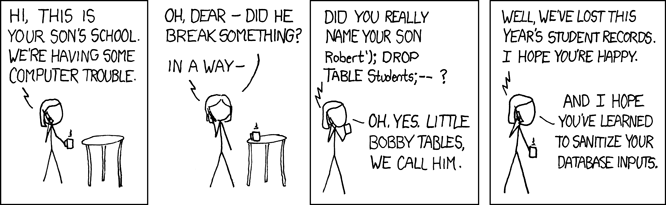
\includegraphics[width=0.7\textwidth]{bobbyTables.png}
			\attribution{XKCD}
		\end{center}
	\end{frame}

	\begin{frame}[fragile]
		\frametitle{Работа с метаинформацией}
		ALTER TABLE:
		\begin{minted}{sql}
ALTER TABLE Students ADD email VARCHAR(MAX);
ALTER TABLE Students DROP COLUMN email;

ALTER TABLE Students ADD PRIMARY KEY (Code);

		\end{minted}
	\end{frame}

	\section{ADO.NET}

	\begin{frame}
		\frametitle{Низкий уровень работы с данными, ADO.NET}
		\begin{itemize}
			\item Возможность исполнять SQL-запросы для разных источников данных
			\item Data Provider обеспечивает общение с конкретной СУБД
			\item Connection String описывает, как подключиться к СУБД
			\item Command представляет абстракцию команды в СУБД
			\item DataSet обеспечивает более-менее высокоуровневое представление данных
			\item Может работать даже с XML или таблицами Excel
			\item Пространство имён System.Data
			\item Лучше не использовать в современном коде
		\end{itemize}
	\end{frame}

	\begin{frame}[fragile]
		\frametitle{Пример, чтение из базы}
		\begin{footnotesize}
			\begin{minted}{csharp}
public static void Main()
{
    using (var connection = new MySqlConnection(
        "database=cities;server=localhost;user id=root;" + 
        "Password=my-secr3t-p4ssw0rd;SslMode=none"))
    {
        var command = new MySqlCommand("SELECT Id, Name FROM City", connection);
        connection.Open();
        var reader = command.ExecuteReader();
        while (reader.Read())
        {
            Console.WriteLine($"Id: {reader.GetInt32(0)}\tName:{reader.GetString(1)}");
        }
    }
}
			\end{minted}
		\end{footnotesize}
	\end{frame}

	\begin{frame}[fragile]
		\frametitle{Пример, добавление в базу}
		\begin{footnotesize}
			\begin{minted}{csharp}
public static async Task Main()
{
    using (var connection = new MySqlConnection(
        "database=cities;server=localhost;user id=root;" +
        "Password=my-secr3t-p4ssw0rd;SslMode=none"))
    {
        var command = new MySqlCommand(
            "INSERT INTO City (name) VALUES (@name)", connection);
        command.Parameters.AddWithValue("@name", "Peterhof");
        connection.Open();
        await command.ExecuteNonQueryAsync();
        Console.WriteLine($"Done, inserted row id = {command.LastInsertedId}");
    }
}
			\end{minted}
		\end{footnotesize}
	\end{frame}

	\section{EF Core}

	\begin{frame}
		\frametitle{Высокий уровень работы с данными, Entity Framework}
		\begin{itemize}
			\item ORM (Object-Realtional Mapping) системы --- преобразуют реляционные данные в объекты
			\item ORM-библиотека берёт на себя общение с базой
			\begin{itemize}
				\item И даже генерацию SQL-запросов
				\item Типобезопасность
			\end{itemize}
			\item Entity Framework Core --- одна из реализаций для .NET (.NET Core)
		\end{itemize}
	\end{frame}

	\begin{frame}
		\frametitle{Как она работает}
		\begin{center}
			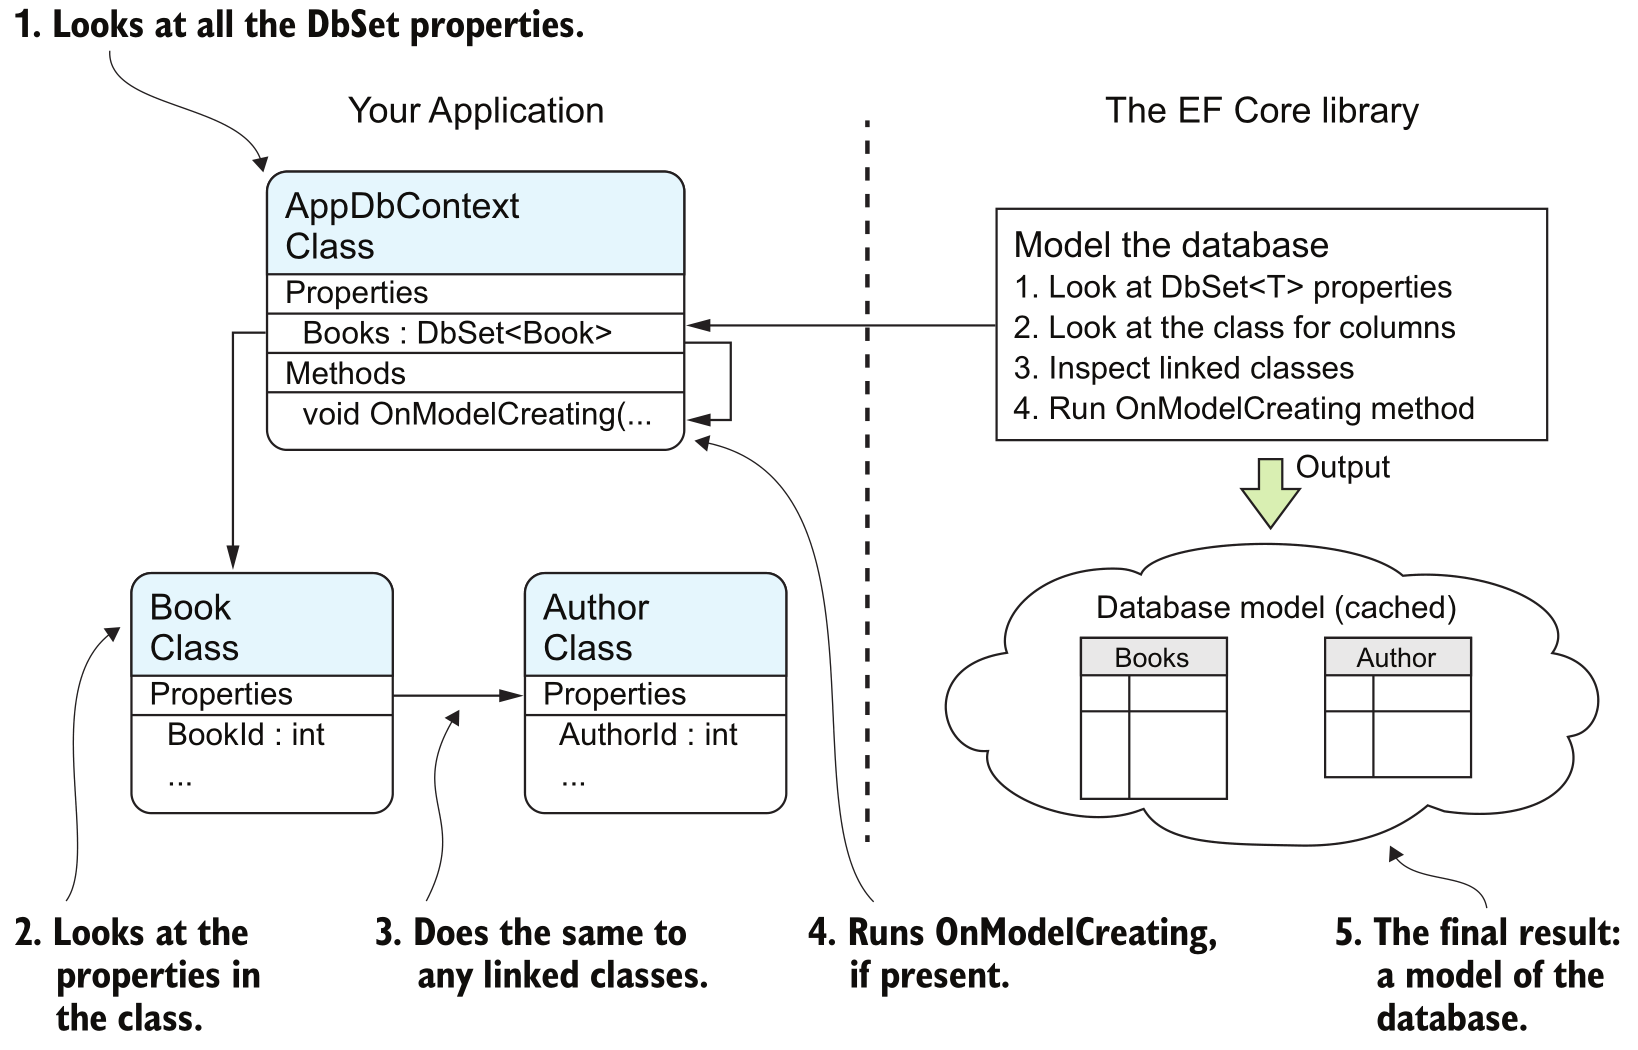
\includegraphics[width=0.85\textwidth]{efCoreDatabaseModeling.png}
			\attribution{J. Smith, ``Entity Framework Core In Action''}
		\end{center}
	\end{frame}

	\begin{frame}[fragile]
		\frametitle{Как это примерно выглядит в коде}
		\framesubtitle{Запрос к базе}
		\begin{footnotesize}
			\begin{minted}{csharp}
public static void ListAll()
{
    using (var db = new AppDbContext())
    {
        foreach (var book in db.Books.AsNoTracking().Include(a => a.Author))
        {
            var webUrl = book.Author.WebUrl == null 
                ? "- no web URL given -" 
                : book.Author.WebUrl;
            Console.WriteLine($"{book.Title} by {book.Author.Name}");
            Console.WriteLine("Published on " 
                + $"{book.PublishedOn:dd-MMM-yyyy}" 
                + $". {webUrl}");
        }
    }
}
			\end{minted}
		\end{footnotesize}
	\end{frame}

	\begin{frame}
		\frametitle{Что в это время делает EF}
		\begin{center}
			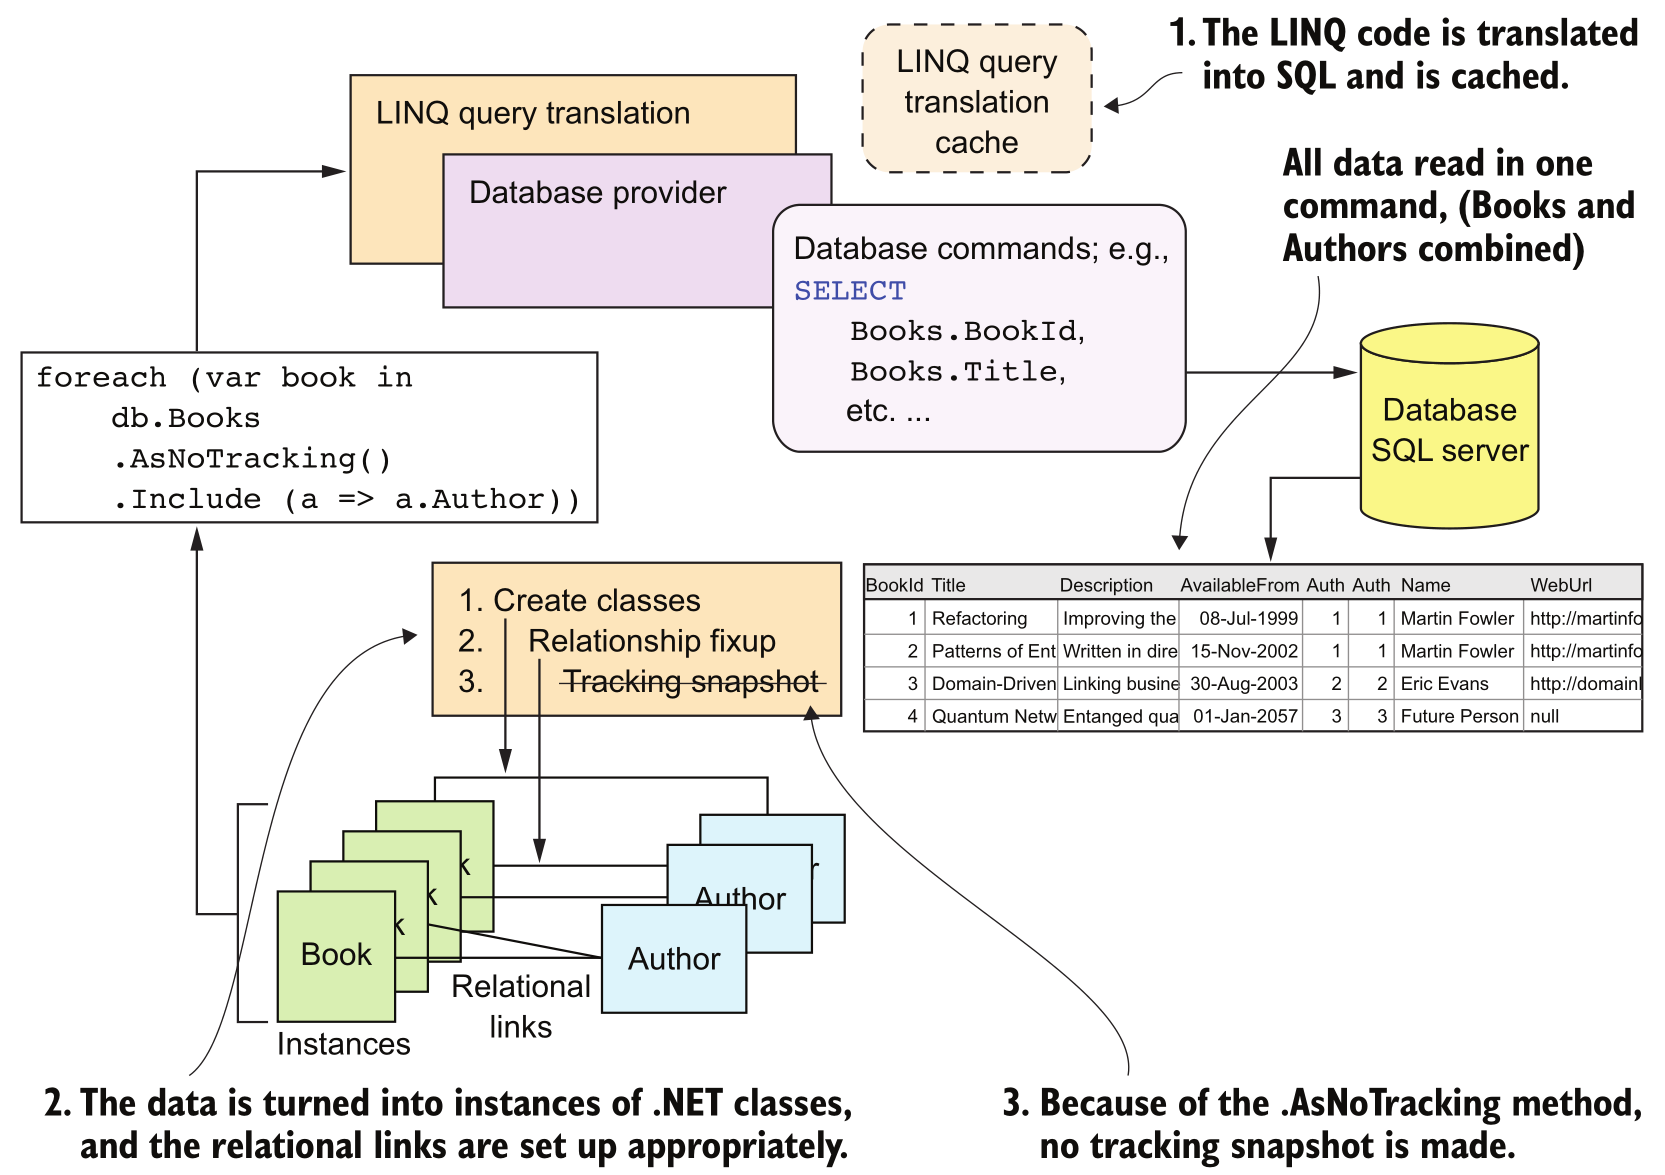
\includegraphics[width=0.8\textwidth]{efCoreQuery.png}
			\attribution{J. Smith, ``Entity Framework Core In Action''}
		\end{center}
	\end{frame}

	\begin{frame}[fragile]
		\frametitle{Сгенерированный SQL}
		\begin{minted}{sql}
SELECT b.BookId,
    b.AuthorId,
    b.Description,
    b.PublishedOn,
    b.Title,
    a.AuthorId,
    a.Name,
    a.WebUrl
FROM Books AS b
INNER JOIN Author AS a ON
    b.AuthorId = a.AuthorId
		\end{minted}
	\end{frame}

	\begin{frame}[fragile]
		\frametitle{Обновление данных}
		\begin{footnotesize}
			\begin{minted}{csharp}
public static void ChangeWebUrl()
{
    Console.Write("New Quantum Networking WebUrl > ");
    var newWebUrl = Console.ReadLine();
    using (var db = new AppDbContext())
    {
        var book = db.Books.Include(a => a.Author)
                           .Single(b => b.Title == "Quantum Networking");
        book.Author.WebUrl = newWebUrl;
        db.SaveChanges();
        Console.WriteLine("... SavedChanges called.");
    }
}
			\end{minted}
		\end{footnotesize}
	\end{frame}

	\begin{frame}
		\frametitle{Что в это время делает EF}
		\begin{center}
			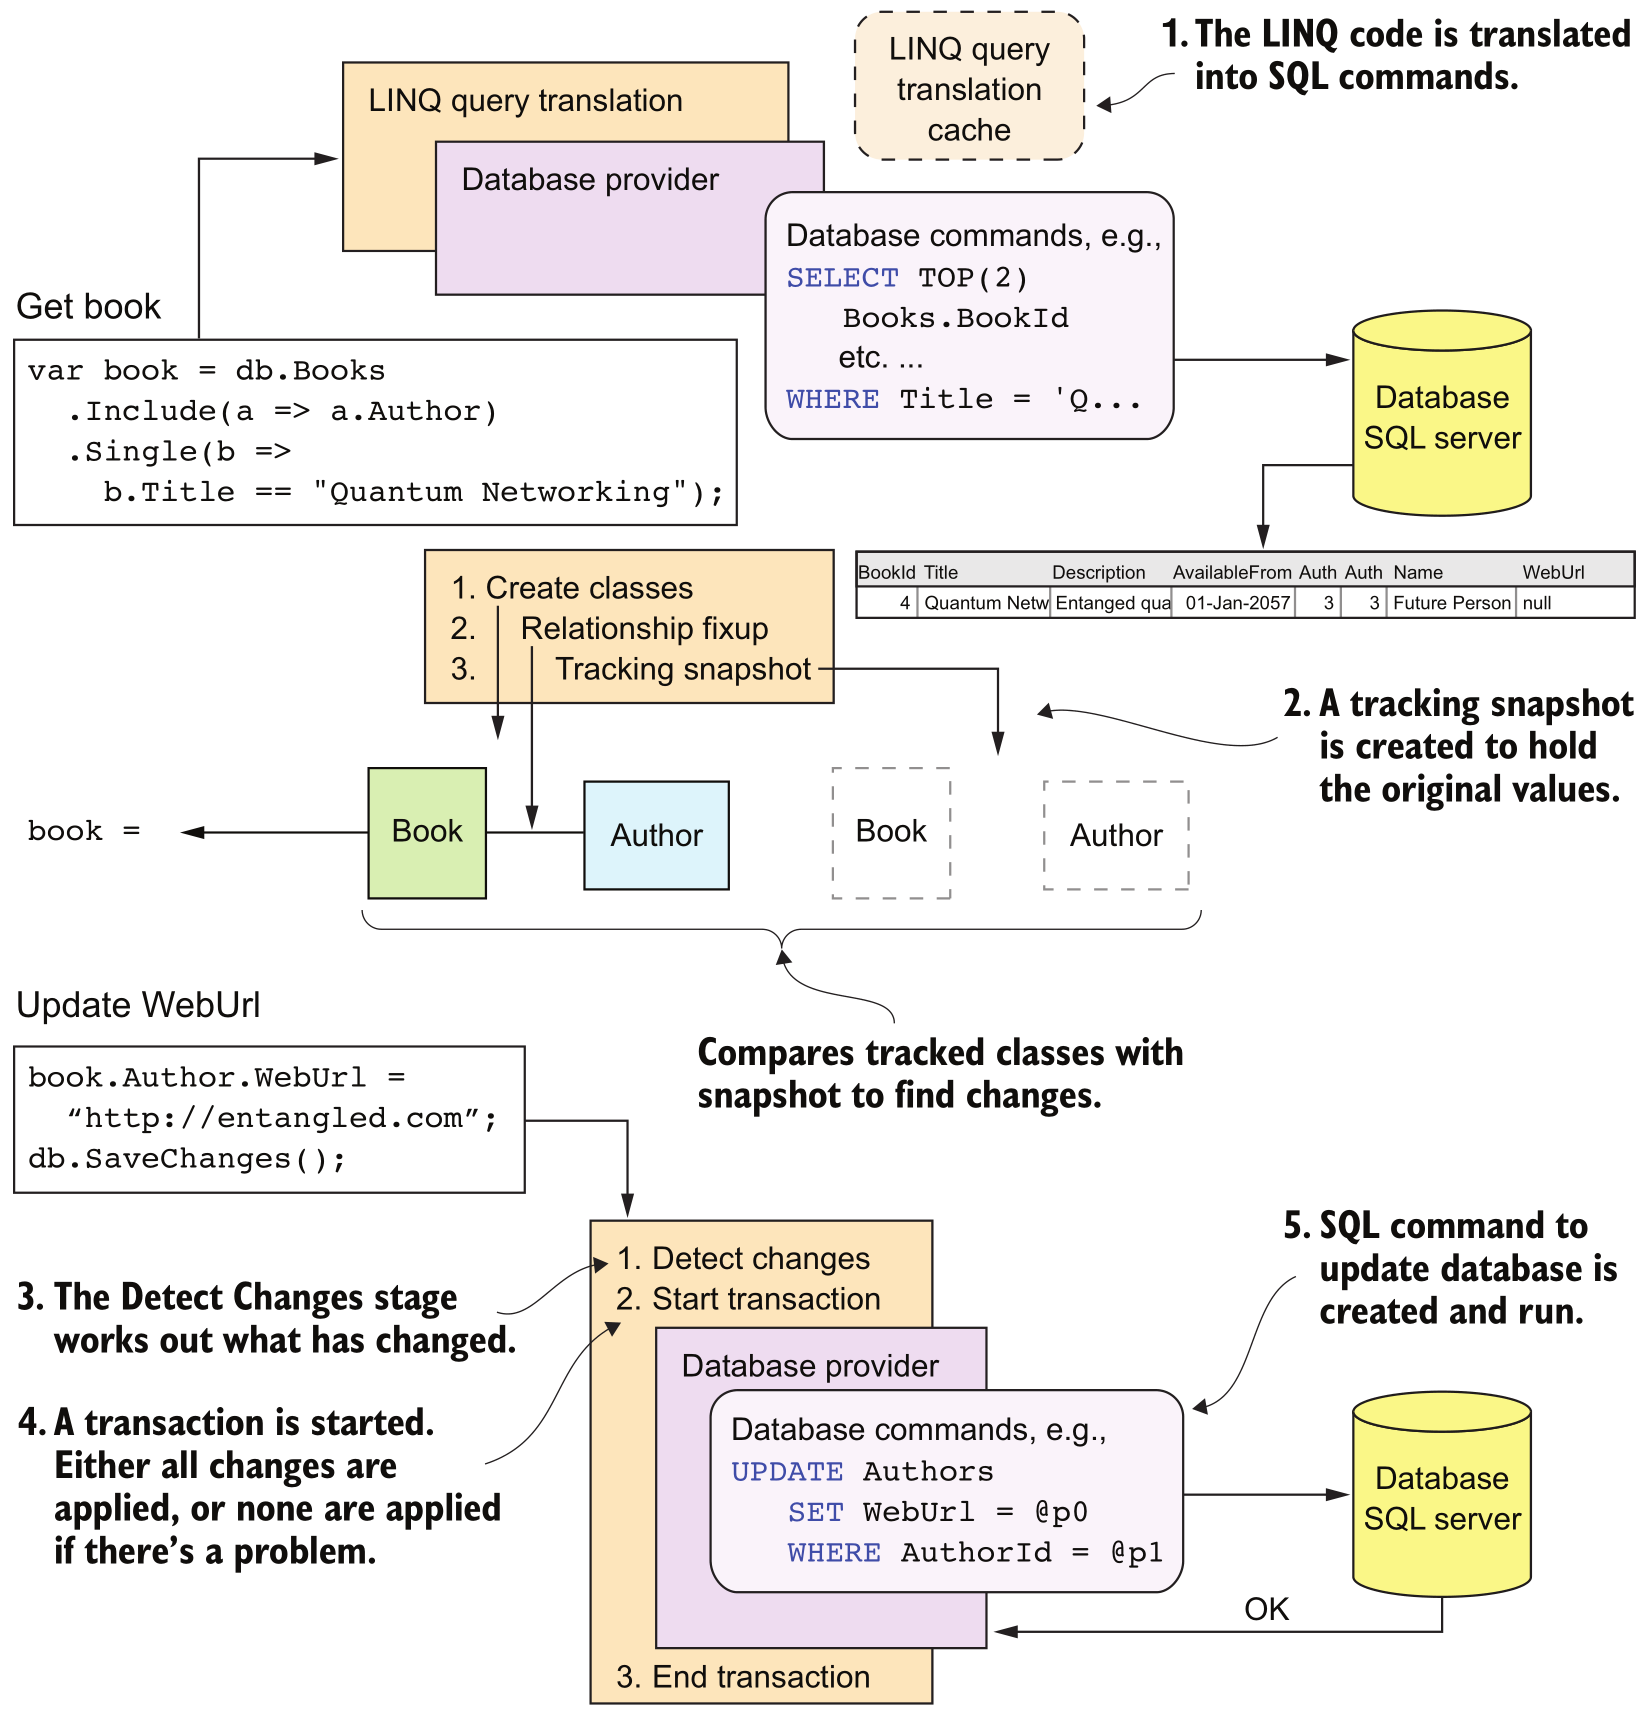
\includegraphics[width=0.5\textwidth]{efCoreUpdate.png}
			\attribution{J. Smith, ``Entity Framework Core In Action''}
		\end{center}
	\end{frame}

\end{document}
